%% LyX 1.3 created this file.  For more info, see http://www.lyx.org/.
%% Do not edit unless you really know what you are doing.
\documentclass[english,12pt,a4paper,twoside]{report}
\usepackage{times}
%\usepackage{algorithm2e}
\usepackage{url}
\usepackage{bbm}
\usepackage[T1]{fontenc}
\usepackage[latin1]{inputenc}
\usepackage{geometry}
%\geometry{verbose,letterpaper,tmargin=2.5cm,bmargin=3cm,lmargin=3cm,rmargin=3cm}
\usepackage{rotating}
\usepackage{graphicx}
\usepackage{amsmath, amsthm, amssymb}
\usepackage{setspace}
\usepackage{lineno}
\usepackage{hyperref}
\usepackage{bbm}

%\usepackage{xcolor,framed}
%\colorlet{shadecolor}{blue!10}
%\begin{shaded}blabla\end{shaded}

%\usepackage{xr}
%\externaldocument{PRS-supp}

%\linenumbers
%\doublespacing
\onehalfspacing
%\usepackage[authoryear]{natbib}
\usepackage{natbib} \bibpunct{(}{)}{;}{author-year}{}{,}


%Pour les rajouts
\usepackage{xcolor}

\usepackage{dsfont}
\usepackage[warn]{textcomp}
\usepackage{adjustbox}
\usepackage{multirow}
\usepackage{graphicx}
\graphicspath{{figures/}}
\DeclareMathOperator*{\argmin}{\arg\!\min}

\let\tabbeg\tabular
\let\tabend\endtabular
\renewenvironment{tabular}{\begin{adjustbox}{max width=0.75\textwidth}\tabbeg}{\tabend\end{adjustbox}}

\makeatletter

%%%%%%%%%%%%%%%%%%%%%%%%%%%%%% LyX specific LaTeX commands.
%% Bold symbol macro for standard LaTeX users
%\newcommand{\boldsymbol}[1]{\mbox{\boldmath $#1$}}

%% Because html converters don't know tabularnewline
\providecommand{\tabularnewline}{\\}
\definecolor{clumping}{HTML}{38761D}
\definecolor{thresholding}{HTML}{1515FF}
%<span style="color:#38761D">Clumping</span> + <span style="color:#1515FF">Thresholding</span>

\usepackage{babel}
\makeatother


\begin{document}

\section{Conclusion and Discussion}

\subsection{Problem of generalization}

Polygenic Risk Scores (PRS) might become a central part in precision medicine. For now, predictive performance for most complex diseases are not good enough to be used in clinical settings. 
A major concern with PRS at the moment is their problem of generalization / transferability in different populations. 
Indeed, most GWAS have included European people only (Figure \ref{fig:GWAS-ancestry}). In 2009, 96\% of individuals included in GWAS datasets were of European ancestry \cite[]{need2009next}. In 2016, still more than 80\% of those individuals were of European descent, with an increase of the inclusion of non-European participants, mostly constituted of Asian people \cite[]{popejoy2016genomics}. People from Hispanic or African ancestry are still poorly represented \cite[]{martin2019clinical}.
This poor heterogeneity in inclusion can be explained by the fact that the more diverse are the population in the data we analyze, the more possible confounders there are to account for in order to avoid spurious results. 

\begin{figure}[htpb]
\centerline{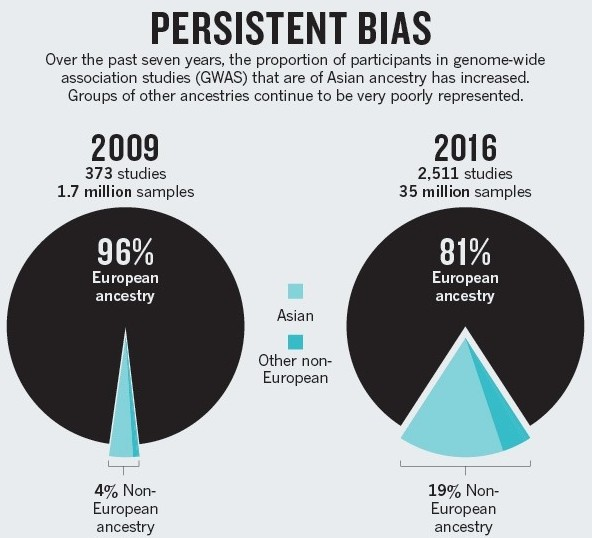
\includegraphics[width=0.6\textwidth]{GWAS-ancestry.jpg}}
\caption{Proportion of GWAS participants by ancestry. Most GWAS include mainly European people, some now include Asian people, but other ethnicities are still poorly represented. Source: \cite{popejoy2016genomics}.}
\label{fig:GWAS-ancestry}
\end{figure}

This lack of heterogeneity in inclusion of diverse populations has several problems. First,
there are some SNP ascertainment bias because SNPs that are more common are more likely to be discovered in GWAS so that discoveries in European tend to have larger frequencies than in other populations, due to the winner's curse. If effects have a frequency that is different between populations, using these effects naturally introduces some shift in PRS distributions for different populations.
Second, rare variants are missed in GWAS if they are specific to some population that is not included in the association study \cite[]{martin2019clinical}. Thus, this limit the predictive ability of PRS in different populations to the one(s) included in the GWAS.
Third, it is accepted that genotyped SNPs, or even imputed SNPs, that are discovered in GWAS may not be the true functional SNPs (fSNPs) having an effect on disease susceptibility. Instead, GWAS are assumed to discover SNPs that tag fSNPs (tagSNPs), i.e.\ are correlated with fSNPs. Yet, LD can be different between populations so that a tagSNP can have a different correlation with the corresponding fSNP, or there can be different fSNPs for different populations. Thus, effects of these SNPs can be different and are often diluted toward zero for populations not included in the GWAS \cite[]{carlson2013generalization}. 
In conclusion, for many reasons, magnitude and frequency of effects can vary considerably between populations, and these differences are larger when populations are more genetically distant such as African population with either European or Asian populations.
These differences in prediction between populations are two-fold (Figures \ref{fig:dist-shift} and \ref{fig:pop-pred}): distributions of PRS are shifted and prediction within each distribution is also reduced \cite[]{vilhjalmsson2015modeling,martin2019clinical}.

\begin{figure}[htpb]
\centerline{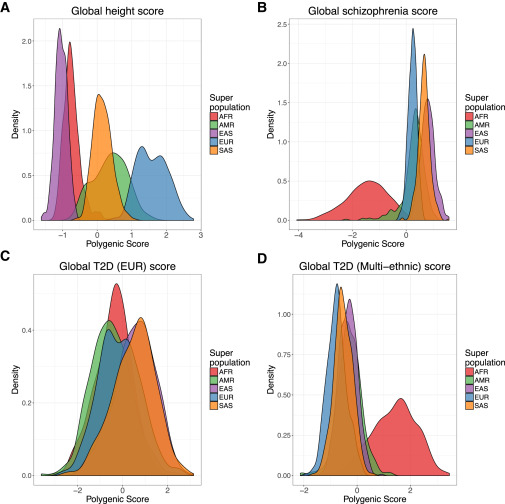
\includegraphics[width=0.6\textwidth]{pred-pops.jpg}}
\caption{Distributions of Polygenic Risk Scores (PRS) for many populations and phenotypes (T2D: Type 2 Diabetes). Source: \cite{martin2017human}.}
\label{fig:dist-shift}
\end{figure}

\begin{figure}[htpb]
\centerline{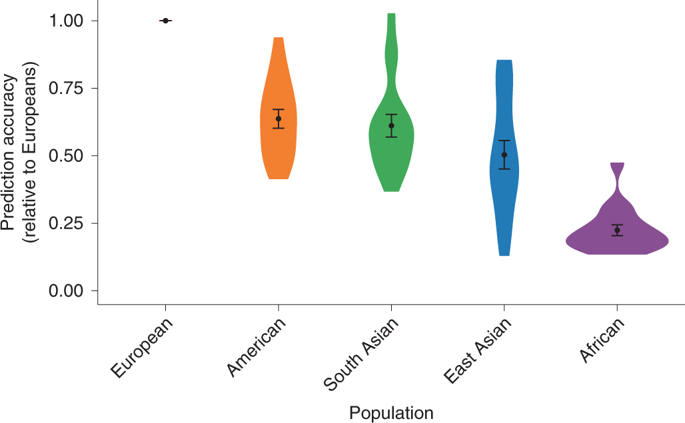
\includegraphics[width=0.7\textwidth]{pop-pred-reduced.png}}
\caption{Prediction accuracy relative to European-ancestry individuals across 17 quantitative traits and 5 continental populations in the UK Biobank data \cite[]{bycroft2017genome}. Source: \cite{martin2019clinical}.}
\label{fig:pop-pred}
\end{figure}


Several solutions have been proposed to partially correct for the differences of prediction between populations. First, \cite{martin2017human} proposed to mean-center PRS for each population, yet this would require an accurate way to assess ancestry and would not work for admixed people, e.g.\ one person with an African father and an European mother \cite[]{reisberg2017comparing}.
Second, it has been suggested to include more diverse population in GWAS \cite[]{pulit2010multiethnic}. Indeed, new associations can be found if the frequency is higher in an under-represented population. 
It would be also possible to fine-map fSNPs in common for multiple populations so that their effects generalize better to any population, irrespective of LD \cite[]{carlson2013generalization,wojcik2018page}.
Finally, statistical methods are starting to emerge in order to use large European GWAS in conjunction with smaller data from another population in order to leverage both the discoveries from the large dataset and the specificities of the smaller dataset \cite[]{marquez2017multiethnic,coram2017leveraging}.


\subsection{Looking for missing heritability in rare variants}

Missing heritability, i.e.\ the gap between heritability estimations from current GWAS studies and from family studies, could reside in rare variants.
Indeed, for height and colorectal cancer, it has been shown that estimations of heritability from GWAS data could recover almost all heritability when a large proportion of low-frequency variants was present in the data \cite[]{yang2015genetic,huyghe2019discovery,wainschtein2019recovery}.
However, actual findings of significantly associated variants of low-frequency are scarce. 
For example, a GWAS of height including more than 700K individuals found 83 associated variants with allele frequencies between 0.1\% and 4.8\%, with effects up to 2 cm per allele \cite[]{marouli2017rare}. Yet, these 83 variants together accounts for only 1.7\% of the total heritability of height. 
In other large studies, one for coronary artery disease and one for type 2 diabetes, there was little evidence of low-frequency variants with large effects \cite[]{nikpay2015comprehensive,fuchsberger2016genetic}.

Associations of rare variants with traits are difficult to find for two reasons. 
First, it is very difficult to impute low-frequency variants with a good quality if using for example a small reference panel such as the 1000 genomes \cite[]{nikpay2015comprehensive}. There is now a reference panel of 32,000 individuals that is used to accurately impute variants with allele frequencies as low as 0.1\% \cite[]{mccarthy2016reference}. 
This large reference panel is European specific, which means that imputing data from other ancestries is more difficult. This is a problem because, one way to discover and accurately estimate the effect of a rare variant is to find it in a population in which its allele frequency is larger. 
Indeed, the power of association studies is dependent on the variance explained by a locus; for example, for a disease that affects 1\% of the population, we have the same power to detect a risk locus of 50\% frequency and odds ratio of 1.1 as we do for a risk locus of 0.1\% frequency and odds ratio of 2.9 \cite{wray2018common}.

The second reason is that sequencing technologies are more expensive than genotypying and imputation. Currently, studies have mostly focused on whole exome sequencing (WES) because it is cheaper than whole genome sequencing (WGS). The exome is also where the effect sizes of variants are expected to be larger and where discoveries are likely to be more immediately actionable \cite[]{zuk2014searching}. Yet, sample sizes of sequencing studies remain small and special considerations and challenges arise when testing rare frequency variants from these studies \cite[]{auer2015rare}.
Thus, sample size is the limiting factor in variant discovery, not genotyping technology \cite{wray2018common}. 
It is probably the limiting factor in prediction too.
[TODO: moreover, too much M formula]


\newpage

\bibliographystyle{natbib}
\bibliography{refs}

\end{document}
